\section{Cyclic closure of the periodic system}\label{sec:06-closure}

The captured periodic groups may still intersect cyclically. We first
join these overlaps to obtain a malnormal system. The next two sections
fold its actual subtrees into lines and enlarge groups when distinct
lines share an end. Throughout, joint injection into $H_1(L;D_L)$ keeps
the total dimension at most $k-1$; the termination arguments must also
control the operations that do not increase this dimension.

We retain the ambient torsion-free hyperbolic primitive extension group
$G$, its height map $h:G\to\mathbb Z$, the height kernel $L$, and the
actual tree $T$ of Section~\ref{sec:03-rows}. Coefficients and transport
of orbit representatives have the conventions of that section. In
particular, $\beta(V)=\dim_{D_V}H_1(V;D_V)$, and all dimensions below are
unchanged on extension to an overfield. A noncyclic subgroup is
\emph{detected} when one of its normalized Fox differences
$\Delta(a)-\Delta(b)$ has nonzero image in $H_1(L;D_L)$.

The actual-row inputs are Lemmas~\ref{row:level-basis},
\ref{row:row-finiteness}, \ref{row:cyclic-dictionary}, and
\ref{row:boundary-gates}, together with
Propositions~\ref{row:restriction}, \ref{row:path-inertia}, and
\ref{row:period-rule}. We also use the support and coset descent
assertions of Theorem~\ref{coeff:support}, the semilinear localization
assertion of Lemma~\ref{coeff:analytic-support}, and the captured
periodic system of Proposition~\ref{gate:capture}. In particular, the field homology of
$L$ has dimension $k-1$, the ambient two-boundary is injective, and
sufficiently long noncyclic actual path stabilizers have already been
captured. All statements below concern this actual tree, even when a
new folded tree is constructed.

\subsection{The closure input and its budget}
\begin{definition}[Admissible periodic system]\label{close:input}
An admissible system is a $G$-invariant set of objects with finitely many
$G$-orbits, whose full stabilizers $A$ satisfy the following conditions.
\begin{enumerate}
\item $h(A)\ne0$; $A$ is quasiconvex in $G$, virtually compact special,
and acyclic over $D_A$.
\item Stabilizers of distinct objects intersect at most cyclically.
\item For $S=A\cap L$, one has $0<\beta(S)<\infty$, every noncyclic
subgroup of $S$ is detected, and the natural map
\[
 \bigoplus_{d\in L\backslash\mathcal D}H_1(S_d;D_L)
       \longrightarrow H_1(L;D_L)
\]
is injective. Representatives and coefficient transports are taken in
the convention of Section~\ref{sec:03-rows}.
\item There is a fixed length such that every noncyclic stabilizer of
an actual path of that length lies wholly in one of the $S_d$.
\end{enumerate}
The system supplied by Proposition~\ref{gate:capture} is admissible.
Its \emph{budget} is
\[
 \mathcal B(\mathcal D)=
       \sum_{d\in L\backslash\mathcal D}\beta(S_d)\le k-1.
\]
This is a finite sum: each $G$-orbit splits into finitely many $L$-orbits
because its stabilizer has nonzero height image.
\end{definition}

We use the same closure operation after each end enlargement. Form a
bipartite graph with the old objects as one class of vertices. The
other class consists of maximal cyclic groups $C\le G$ meeting at
least two old stabilizers nontrivially; join $C$ to precisely those
objects it meets. The action at cyclic vertices is conjugation.

\begin{lemma}[The cyclic incidence forest]\label{close:join-forest}
The cyclic incidence graph has finitely many $G$-orbits of edges and is
a forest.
\end{lemma}

\begin{proof}
Quasiconvex double-coset finiteness gives finitely many incidence-edge
orbits. Suppose that a simple circuit has successive old vertices
$A_i$ and cyclic vertices $C_i$, with indices read cyclically. Choose
$1\ne c_i\in C_i\cap A_i\cap A_{i+1}$. Such a common power exists
because both intersections with $C_i$ are nontrivial. We will obtain a
contradiction from one endpoint of the normalized path for $c_i$.

Use literal Fox chains based at the identity, with the same word for
$c_i$ in its two occurrences. Put
\[
 E_i=D_{A_i}\otimes_{\mathbb QA_i}\mathbb QG
       =\sum_{g\in G}D_{A_i}g.
\]
The difference $\Delta(c_i)-\Delta(c_{i-1})$ is a cycle over $E_i$.
Shapiro's lemma and the field acyclicity of the old group $A_i$ give
a finite two-chain $b_i$ over this induced module with
\[
 \partial_2 b_i=\Delta(c_i)-\Delta(c_{i-1}),
 \qquad \sum_i b_i=0.
\]
The second equality follows because the boundaries telescope and
the ambient two-boundary is injective.

Apply the single scalar-function map $\mathcal F$ of
Theorem~\ref{coeff:support}(ii) to every coefficient. It commutes with
the polynomial boundary matrices. Each coefficient of $b_i$ belongs
to a finite sum of $D_{A_i}g$, so its function support lies in a fixed
neighborhood of $A_i$. The pointwise equality $\sum_i\mathcal F(b_i)=0$
then confines the support of each summand to the union of the pairwise
coarse intersections with the other $A_j$. For this finite family,
each such coarse intersection lies in a bounded neighborhood of
$A_i\cap A_j$. Indeed close pairs in the two groups have finitely
many possible discrepancies, and pairs with one fixed discrepancy
form one orbit under $A_i\cap A_j$. Choosing representatives of
those finitely many orbits gives the claimed bound.

Old admissibility makes every $A_i\cap A_j$ cyclic or trivial.
Consequently these function two-chains are supported, outside a
bounded set, near finitely many periodic axes. Group together axes
with the same endpoints. The remaining endpoint directions separate
outside every sufficiently large ball: distinct maximal cyclic groups
in a torsion-free hyperbolic group share no endpoint.

To see the flux on one of these directions explicitly, write
$p_n=\mathcal F((c_i-1)^{-1})(c_i^n)$. Support preservation and right
equivariance give
\[
 p_{n-1}-p_n=\delta_{n,0}.
\]
Thus the values on the two half-orbits are constants $p_-,p_+$ with
$p_--p_+=1$. Choose a half-orbit on which the constant is nonzero.
The corresponding tail of $\mathcal F(\Delta(c_i))$ is a nonzero
constant sum of translates of the chosen word path for $c_i$.
Since $C_{i-1}\ne C_i$, the term $\Delta(c_{i-1})$ has no tail in
this endpoint direction. No positivity or one-sided support of
$\mathcal F((c_i-1)^{-1})$ is needed.

Let $R$ bound the propagation of the boundary matrices. Beyond a
large ball, the distinct endpoint support clusters just described
are more than $2R$ apart. Retain from $\mathcal F(b_i)$ the entire
cluster in the chosen direction beyond that ball, obtaining a
function two-chain $b_i^+$. A selected coefficient and an omitted
coefficient can contribute to the same boundary edge only near the
cutoff ball. In particular all cancellations along the sides of the
selected cluster remain intact. Therefore
\[
 \partial_2 b_i^+
   =\text{the chosen nonzero constant half-ray of word paths}
      +\text{a finitely supported one-chain}.
\]
The correction is finite because the Cayley complex is locally finite
and the boundary matrices have finite propagation. The half-ray has
divergence of nonzero total mass, whereas the divergence of any
finitely supported one-chain has total mass zero. This contradicts
$\partial_1\partial_2b_i^+=0$ and rules out the circuit.
\end{proof}

\begin{lemma}[Component groups before the injection step]\label{close:join-components}
Let $A'$ be the full stabilizer of a component of the cyclic incidence
forest, and put $S'=A'\cap L$. Then $A'$ is finitely generated,
quasiconvex in $G$, virtually compact special, and field-acyclic;
$h(A')\ne0$ and $0<\beta(S')<\infty$. Stabilizers of different new
components intersect at most cyclically. If $e_+$ and $c_+$ count,
modulo $S'$, the incidences and cyclic vertices with nonzero height
image, respectively, then
\begin{equation}\label{close:join-dimension}
 \beta(S')=\sum_{v\in S'\backslash\mathrm{Old}}
                    \beta(S_v)+e_+-c_+.
\end{equation}
Here the old vertex groups are understood in their actual conjugate
positions. No joint ambient injection for the new system is assumed
in this lemma.
\end{lemma}

\begin{proof}
The finite quotient of the incidence forest makes $A'$ a finite graph
of groups with old vertex groups and maximal cyclic vertex groups.
Its edge groups are nontrivial cyclic. The Bass--Serre homology
sequence therefore gives field acyclicity, and the same finite graph
of finitely generated groups gives finite generation. Also
$h(A')\ne0$, since $A'$ contains an old group.

For $S'=A'\cap L$, each old vertex orbit still splits into finitely
many orbits, because the old group has nonzero height image. The
same holds for the nonhorizontal cyclic vertices and incidences.
Horizontal cyclic stabilizers have zero $H_0$ and $H_1$ over their
subgroup fields. At a nonhorizontal cyclic vertex or incidence the
$S'$-stabilizer is trivial, and contributes one dimension in $H_0$.
The tree sequence, with direct sums even when the quotient is infinite,
thus gives exactly
\[
 \beta(S')=\sum_{v\in S'\backslash\mathrm{Old}}\beta(S_v)+e_+-c_+.
\]
It is positive and finite. The period rule and the subtree gate
criterion now give quasiconvexity of $A'$. Its cyclic edge groups
are ambient quasiconvex, so its finite splitting over old VCS vertex
groups gives VCS by the quasiconvex hierarchy theorem
\cite{Wise2021}.

We next control intersections; this must precede the new joint
injection. For any two field-acyclic quasiconvex VCS groups $B,C$
obtained here, their intersection $V$ is quasiconvex and separable in
each. The finite-span assertion of Theorem~\ref{coeff:support} gives
\[
 \left(\sum_gD_Bg\right)\cap\left(\sum_gD_Cg\right)
       =\sum_gD_Vg.
\]
A cycle over the induced $D_V$-module has fillings over both modules
on the left. Ambient two-boundary injectivity makes those fillings
equal, and the displayed equality puts their coefficients in the
module on the right. Shapiro therefore gives $H_1(V;D_V)=0$.
The same induced injectivity gives $H_2(V;D_V)=0$, and $H_0=0$
when $V\ne1$. Thus every nontrivial such intersection is field-acyclic.

Apply this first to $A'$ and an old group from another component.
Their intersection has trivial stabilizers on the join tree: any
nontrivial intersection with an old node or its cyclic neighbor
would join that old group to the component. It is therefore free;
its zero first field homology makes it at most cyclic.

Finally the intersection of two distinct new component groups has
at most cyclic old-node stabilizers. At an old node, any nontrivial
such stabilizer lies in its unique maximal cyclic germ, and hence in
the corresponding incidence stabilizer. Collapse the resulting
nontrivial-edge stars. The intersection is free, and its field
acyclicity again makes it at most cyclic. This supplies the
intersection hypothesis for the next join forest without using the
joint injection to be proved next.
\end{proof}

\begin{lemma}[Detection under cyclic joins]\label{close:join-detection}
Every noncyclic subgroup of a new height kernel $S'$ is detected in
$H_1(S';D_{S'})$. Its image will therefore be detected in ambient
homology once the joint injection below is established.
\end{lemma}

\begin{proof}
We first treat a horizontal piece and then the free-product joins.
On the tree of \(S'\), split along trivial-stabilizer edges (including
positive-height joins), into free product pieces. In horizontal
pieces edge and cyclic node \(H_0,H_1\) vanish, leaving the direct
sum of old vertex \(H_1\)'s. For a noncyclic subgroup contained in
such a piece, if elliptic use old detection.

Otherwise take two independent hyperbolics \(x,y\) with axes strictly on opposite branches from a chosen old node \(v\) (take sufficiently separated translates/conjugates). This is possible because the tree action is acylindrical (successive turns through two distinct maximal cyclic nodes have trivial path stabilizer); elementary nonelliptic actions of subgroups there are virtually cyclic. Indeed end or line stabilizers have trivial kernel of tail translations (respectively, after preserving orientation on a line), and an all-elliptic subgroup has a fixed vertex or fixes tails towards an end. Independent hyperbolics give as widely separated axes as desired, by translating one by large powers of the other (their axis projections to the latter are bounded).

Choose a nonzero \(c\) in the first edge group along \([v,xv]\); the last has \(xcx^{-1}\). Telescope the normalized paths \(\Delta(c_j)\) of arbitrary edge-group elements along this segment with those two terminal choices. Each difference is an internal vertex cycle (cyclic vertices contribute zero); and the entire sum over \([v,xv]\) is
\[
           \Delta(xcx^{-1})-\Delta(c)=(x-1)(\Delta(c)-\Delta(x))
\]
in affine chain coordinates modulo boundaries.

This writes \(\Delta(x)\) as \(\Delta(c)\) plus normalized cycle contributions at the internal nodes. Likewise for \(y\) with a noncommensurable incident cyclic element \(c'\). Thus in the coordinates of the old summand orbit of \(v\), the cycle \(\Delta(x)-\Delta(y)\) contains \(\Delta(c)-\Delta(c')\) at the identity coset; all internal pieces have coefficients supported in products \(\langle x\rangle s S_v\) or \(\langle y\rangle s S_v\) disjoint from \(S_v\) (no translated path interiors revisit that node). By disjoint support and bases over \(D_{S_v}\), equality to zero would force \(\Delta(c)=\Delta(c')\) in that old summand, impossible by induction (equality for generators collapses the entire affine cycle space of their subgroup).

For the trivial-edge free-product splitting, an elliptic noncyclic subgroup uses the injected vertex homology. Otherwise its action is nonelementary: trivial edge stabilizers make an elementary nonelliptic subgroup cyclic. Choose two hyperbolics \(x,y\) with axes on opposite sides of a separating edge, away from its midpoint \(q\). The based segment chain \([q,hq]\) in free edge coordinates is a derivation, so vanishing of a normalized difference in homology would also kill this normalized path difference.

Read the oriented half-edge \(E\) from \(q\) towards the \(x\)-axis. Only \(E,xE\) from \(\langle x\rangle E\) occur along \([q,xq]\), as first and reversed last: these are the axis hairs with distinct attachment points. No \(\langle y\rangle E\) occurs on \([q,yq]\). The two contributions for \(x\) give coefficient \(-1\) on normalization, which other pieces cannot cancel by disjoint support, since these edge stabilizers are trivial. Thus the normalized difference is nonzero, proving detection in \(H_1(S')\).
\end{proof}

\begin{proposition}[Joint injection after a cyclic join]\label{close:join-injection}
For the new component system the map
\[
 \bigoplus_{i\in L\backslash\mathcal D'}H_1(S'_i;D_L)
       \longrightarrow H_1(L;D_L)
\]
is injective. Consequently a cyclic-join round preserves
admissibility and does not decrease the budget. A round containing a
positive-height cyclic join increases the budget by at least one.
\end{proposition}

\begin{proof}
Write $\mathcal D'$ for the new component system, and let
\[
 V=\ker\left(\bigoplus_{i\in L\backslash\mathcal D'}
       H_1(S_i';D_L)\longrightarrow H_1(L;D_L)\right).
\]
There are three trees in the argument: the current join forest
computes these homologies, the next join forest receives localized
coefficients, and one level of the actual tree $T$ supplies independent
chain columns. Lemma~\ref{close:join-components} makes the next forest
available before the current joint injection has been established.

In the current Bass--Serre sequence, old joint injection makes the
map from $V$ to the sum of the positive-height-edge $H_0$ coordinates
injective. The old vertex orbits summed here are exactly the old
$L$-orbits. Choose a common positive height $b$ for all these finitely
many orbit coordinates. At a component $i$, height transport uses an
element $g_i\in A_i'$ with $h(g_i)=b$ and acts on coefficients by
conjugation followed by left multiplication by $t^bg_i^{-1}$.
Inner transport on homology equals left multiplication, so this action
is independent of the chosen lift and respects the tree sequence.
At a positive-height edge we may instead choose its stabilizer
element $g$ of height $b$; its coordinate action is
\[
 p\longmapsto t^bpg^{-1}.
\]
Each one-dimensional coordinate is simple over the skew Laurent ring.
Their finite direct sum is semisimple. If $V\ne0$, it therefore
contains a simple submodule whose nonzero projection onto one
coordinate is an isomorphism. Normalize its generator to have
coordinate $1$. Its height translate is $t^bg^{-1}$ times itself.

Choose an intrinsic $D_{S_i'}$-basis at every component, and let $B_i$
be the matrix of transport by $g_i$, including its action on
coefficients. A coefficient row $\lambda_i$ of the chosen vector
then satisfies
\[
 t^b\lambda_i g_i^{-1}B_i=t^bg^{-1}\lambda_i,
 \qquad
 g\lambda_i g_i^{-1}=\lambda_iB_i^{-1}.
\]
Lemma~\ref{coeff:analytic-support} localizes these rows to finitely
many cosets whose transporters conjugate the contributing objects
into one component of the next cyclic-join forest: their stabilizers
share powers of $g$. Denote its group by $A^*$ and its height kernel
by $S^*=A^*\cap L$.

For each nonzero row choose one of its height-zero transporters $x_i$
as the new representative. Any other contributing transporter $x$
has $xx_i^{-1}\in S^*$: it sends the same object into the same next
component and has height zero. Also $x_iS_i'x_i^{-1}\le S^*$.
Conjugating the basis cycles by $x_i$ and replacing their coefficients
by $\lambda_i x_i^{-1}$ therefore puts the sum over
$\mathcal U(S^*)$, without changing its ambient class. Distinct
selected indices remain distinct vertex orbits in the next tree,
since an $S^*$-identification would already identify their old
$L$-orbits. Edge first homology is zero in that tree, so its
Bass--Serre sequence makes the resulting sum nonzero in
$H_1(S^*;\mathcal U(S^*))$. Scalar extension is flat here because
each intrinsic coefficient ring is a division ring.

Use the period rule to represent each contributing intrinsic basis
at one fixed actual $P$-row level. This replacement differs from the
old representative by a boundary over $D_{S_i'}$. After conjugation
and extension it is still a boundary over $\mathcal U(S^*)$ in the
induced complex, so the nonzero class just obtained is preserved.
All $x_i$ have height zero, and the period rule holds at every level;
thus these representatives use one common interval of horizontal
$a$-columns. Connecting frame chains cancel on cycles.

Their ambient class is zero by the definition of $V$. Independence
of the columns at this actual free-row level makes their literal
sum zero. This equality already holds in the restricted induced
complex: for finitely many affiliated coefficients a common
invertible affiliated multiplier makes them bounded, after which
distinct $S^*$-cosets have disjoint Fourier supports. This is coset
independence for $\mathcal U(S^*)\cdot L$. It contradicts the
nonzero class in $H_1(S^*;\mathcal U(S^*))$, proving $V=0$.

At a positive-height cyclic node of degree $m\ge2$, the dimension
formula in Lemma~\ref{close:join-components} adds $m-1$ to the old
total. Horizontal nodes add zero. Detection and capture are preserved
by the preceding lemmas and containment of the old kernels. Hence
admissibility is preserved, the budget does not decrease, and a
positive-height join increases it by at least one.
\end{proof}

\begin{proposition}[Finite strict closure]\label{close:strict-system}
Iterating cyclic joins stops after finitely many rounds. The final
system is admissible and strictly malnormal: stabilizers of distinct
objects have trivial intersection. Each is the full stabilizer of its
object. For each final object $d$, the union of all actual rows $x$
with $X_x\cap S_d\ne1$ is a connected subtree $Z_d$ with finite
$D_d$-quotient, where $D_d$ is its object stabilizer and $S_d=D_d\cap L$.
\end{proposition}

\begin{proof}
Every round containing a positive-height join raises the injected
integer dimension, which is at most $k-1$. There can therefore be
only finitely many such rounds. We must separately show that an
infinite sequence of horizontal joins cannot remain after them.

Follow a nested chain of component groups and put
\[
 A^\infty=\bigcup_n A_n,\qquad
 S^\infty=A^\infty\cap L,\qquad
 M_x^\infty=S^\infty\cap X_x.
\]
Homology commutes with this increasing union, and joint ambient
injection gives $0<\beta(S^\infty)\le k-1$. Also $h(A^\infty)\ne0$.
The homology part of the period rule consequently applies before
finite generation is known. Let $Y$ be the convex hull of the rows
with noncyclic $M_x^\infty$. Every edge of $Y$ has nontrivial
$S^\infty$-stabilizer.

Consider a finite run in $Y$ on which the $M_x^\infty$ are cyclic.
Successive edge stabilizers are commensurable in each intervening
cyclic $M_x^\infty$, so one nonidentity power $c\in S^\infty$
fixes the whole run. If a subblock of the fixed capture length has
noncyclic \emph{ambient} actual stabilizer $K$, then $K$ lies in an
originally captured kernel. Choose a stage $n$ containing $c$ on
our chain and follow that captured object's descendant to the same
stage. Both stage-$n$ groups contain $c$, so they coincide or join
at the next round. Thus $K\le S^\infty$. The rows of this block
would then have noncyclic $M_x^\infty$, a contradiction. All such
subblocks therefore have cyclic ambient stabilizer, and the cyclic
path dictionary bounds the length of the run uniformly.

We now build a finite quotient of $Y$. The level homology bound and
height periodicity give finitely many $A^\infty$-orbits of rows with
noncyclic $M_x^\infty$. Every $M_x^\infty$ has finite beta by row
restriction, hence is finitely generated and quasiconvex in $X_x$
by Lemma~\ref{row:row-finiteness}. Quasiconvex double-coset finiteness,
applied to the finitely many actual incident-edge types in $X_x$,
gives finitely many incident orbits with nontrivial intersection.
The uniform bound on intervening cyclic runs means that every row
of the hull is reached within bounded distance of a noncyclic row.
Induction over that distance, using the finite local orbit lists,
proves that $A^\infty\backslash Y$ is finite. Its stabilizers are
finitely generated, so $A^\infty$ is finitely generated.

A finite generating set of $A^\infty$ belongs to one stage; the
chain equals its union from that stage onward. No further distinct
object can merge into a stationary component: it would bring a
noncyclic old group previously meeting that component group at most
cyclically. Every component descends from one of finitely many
initial orbit representatives, so stationarity is simultaneous.
The final objects have trivial pairwise stabilizer intersections and
have full stabilizers by construction.

For completeness, in this strict state let $Y_d$ be the noncyclic
hull for $S_d$. If an actual row $x$ has $X_x\cap S_d\ne1$, any
nontrivial element of that intersection fixes the bridge from $x$
to $Y_d$. A noncyclic ambient capture block on the part outside
$Y_d$ would belong to some $S_{d'}$; its common bridge element forces
$d'=d$ by strictness, contradicting its position outside the hull.
The cyclic dictionary therefore bounds the length of the bridge.
Finite local orbit branching gives a finite quotient after adding
all these rows. The union is connected, since every point of each
bridge also has nontrivial intersection with $S_d$. This is $Z_d$.
\end{proof}

\section{Strict row folding}\label{close:strict-folds}

Cyclic closure has produced a strict system and its actual subtrees
$Z_d$. We identify points at equal height within each $Z_d$, sending it
to a line. The task is to prove that this quotient remains a tree and
that its rows and incident-edge maps retain the homology injections
needed to control path stabilizers.

\subsection{Subtrees and horizontal fibers}

\begin{lemma}[Root closure and the enlarged actual subtrees]\label{close:strict-subtrees}
In a strict system, each $D_d$ is root-closed in $G$. Its subtree
$Z_d$ consists exactly of the actual rows with
$M_x^d=X_x\cap S_d\ne1$, and has finite $D_d$-quotient. At every actual
level the sum of the homologies of the $M_x^d$, over $S_d$-orbits, maps
isomorphically onto $H_1(S_d)$. At an actual vertex the analogous sum
over one slot maps isomorphically onto $H_1(M_x^d)$.
\end{lemma}

\begin{proof}
If $g^m\ne1$ belongs to $D_d$, it also belongs to
$gD_dg^{-1}=D_{gd}$. Strictness forces $gd=d$, hence $g\in D_d$.
Thus $D_d$ is root-closed. Proposition~\ref{close:strict-system}
constructed $Z_d$ from all rows with nontrivial $M_x^d$ and proved
its finite quotient. The period rule identifies the sum at each
actual level with $H_1(S_d)$. Its adjacent-level equality,
restricted to the summands at one actual vertex, gives the stated
local slot equality.
\end{proof}

Equate points of each \(Z_d\) at the same height, and take the transitive quotient of \(T\). It is a tree \(\widehat T\), with the same maximal-orbit types as before (one orbit at each level under \(L\)), and each \(Z_d\) maps onto a monotone line \(\ell_d\).

Indeed its image has one point per height, and any circuit in the quotient lifts after adding connecting paths in the \(Z_d\)'s which project to backtracks.

At a vertex or mid-edge level the components before identification are described by the bipartite graphs \(\Gamma_w\), with nodes the actual rows \(x\) and the \(d\)'s over \(w\), and an edge when \(x\in Z_d\). Here \(w\) denotes one resulting folded place (row position in \(\widehat T\)); \(Y_w=\operatorname{Stab}_G(w)\le L\). 
The coefficient transport conventions remain in force after folding.
In particular $Y_w$ is always a subgroup of $L$.

Figure~\ref{fig:row-refinement-folding} shows the strict folding and
its horizontal incidence data. The tree and homology assertions needed
for this construction are proved below.
\begin{figure}[tbp]
\centering
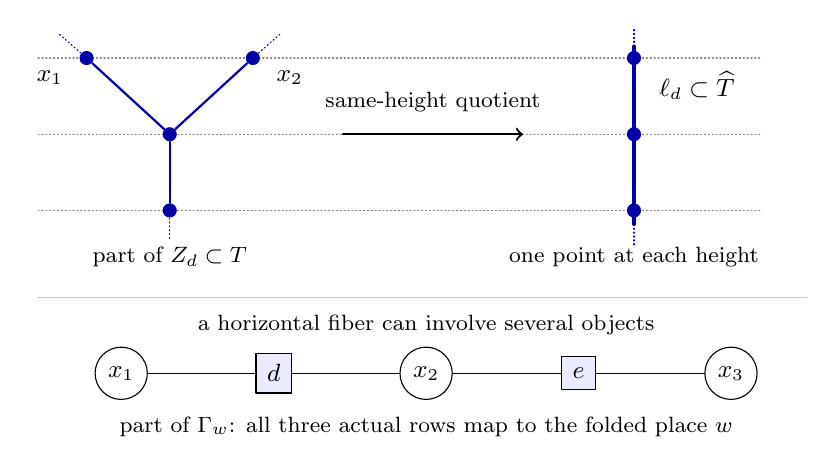
\begin{tikzpicture}[x=.88cm,y=.88cm,font=\small,
  every node/.style={align=center},line cap=round,line join=round,
  row/.style={draw,circle,fill=white,inner sep=3pt},
  object/.style={draw,rectangle,fill=blue!8,inner sep=4pt},
  dot/.style={circle,fill=blue!65!black,inner sep=1.8pt}]
  \draw[densely dotted,gray] (.4,-.15)--(10.85,-.15);
  \draw[densely dotted,gray] (.4,-1.25)--(10.85,-1.25);
  \draw[densely dotted,gray] (.4,-2.35)--(10.85,-2.35);
  \node[dot] (za) at (1.1,-.15) {};
  \node[dot] (zb) at (3.5,-.15) {};
  \node[dot] (zc) at (2.3,-1.25) {};
  \node[dot] (zd) at (2.3,-2.35) {};
  \draw[thick,blue!65!black] (za)--(zc)--(zb);
  \draw[thick,blue!65!black] (zc)--(zd);
  \draw[densely dotted,blue!65!black] (za)--(.7,.2);
  \draw[densely dotted,blue!65!black] (zb)--(3.9,.2);
  \draw[densely dotted,blue!65!black] (zd)--(2.3,-2.78);
  \node[anchor=east] at (.9,-.43) {$x_1$};
  \node[anchor=west] at (3.7,-.43) {$x_2$};
  \node[font=\footnotesize] at (2.3,-3.02) {part of $Z_d\subset T$};
  \draw[->,thick] (4.8,-1.25)--(7.4,-1.25);
  \node[fill=white,inner sep=2pt,font=\footnotesize] at (6.1,-.78)
    {same-height quotient};
  \draw[very thick,blue!65!black] (9,-2.55)--(9,.02);
  \draw[densely dotted,blue!65!black] (9,-2.55)--(9,-2.85);
  \draw[densely dotted,blue!65!black] (9,.02)--(9,.28);
  \node[dot] at (9,-.15) {};
  \node[dot] at (9,-1.25) {};
  \node[dot] at (9,-2.35) {};
  \node[anchor=west,fill=white,inner sep=2pt] at (9.28,-.55)
    {$\ell_d\subset\widehat T$};
  \node[font=\footnotesize] at (9,-3.02) {one point at each height};

  \draw[gray!45] (.4,-3.6)--(11.5,-3.6);
  \node[font=\footnotesize] at (6,-4.0)
    {a horizontal fiber can involve several objects};
  \node[row] (x1) at (1.6,-4.7) {$x_1$};
  \node[object] (d) at (3.8,-4.7) {$d$};
  \node[row] (x2) at (6,-4.7) {$x_2$};
  \node[object] (e) at (8.2,-4.7) {$e$};
  \node[row] (x3) at (10.4,-4.7) {$x_3$};
  \draw (x1)--(d)--(x2)--(e)--(x3);
  \node[font=\footnotesize] at (6,-5.47)
    {part of $\Gamma_w$: all three actual rows map to the folded place $w$};
\end{tikzpicture}
\caption{Strict folding is the transitive quotient generated by identifying
same-height points within each $Z_d$. The upper panel shows the image
of one subtree; horizontal guides indicate height. It does not identify
arbitrary equal-height points of $T$. The lower panel records how two
objects can make three actual rows equivalent at one height: an incidence
$x,d$ means $x\in Z_d$. Such incidence chains describe the horizontal
fiber $\Gamma_w$, whose stabilizer and homology are analyzed below.}
\label{fig:row-refinement-folding}
\end{figure}


\begin{lemma}[Raw horizontal jump vectors]\label{close:raw-jumps}
Fix an actual row group $X$ at a given level, and represent its actual
rows by frame cosets $pX\subset L$. A jump from $pX$ to $qX$ through
one object $d$ has a raw horizontal one-chain representative with
divergence $q-p$. Its coefficient support is contained both in a
finite union of $S_dr$ and in the union of the actual $X$-cosets
incident to $d$. Root-row representatives are taken before eliminating
the root relation.
\end{lemma}

\begin{proof}
The support assertion uses Theorem~\ref{coeff:support}. Fix an actual group \(X\) of the given level, using its one-chain generators in the horizontal Fox quotient of \(L\); rows now have frame cosets \(pX\) in \(L\). We use raw vectors on those generators, i.e. before eliminating the root relation if there is one. For any jump \(pX\to qX\) through \(d\), take \(1\ne a\in S_d\cap pXp^{-1}\), \(1\ne b\in S_d\cap qXq^{-1}\). The difference \(d(q)-d(p)\) (here the symbol on group elements denotes Fox chains) is represented by a raw vector obtained as
\[
 q\Delta_X(q^{-1}bq)-p\Delta_X(p^{-1}ap) -
       (\Delta(b)-\Delta(a)).
\]
For the last parenthesis use an expression by cycles from the \(M_x^d\) in the current level, with coefficients over \(D_{S_d}\), possible by the period isomorphism. In moving any such cycle from a conjugate row to its horizontal coordinates the frame chain terms cancel. In particular each may be written by differences of normalized elements just as in this formula, since such differences span the intrinsic cycle space modulo 2-boundaries for a nontrivial group. This proves the representation assertion by the conjugation rule. All coefficients are thus supported (in the sense of Theorem~\ref{coeff:support}) in finite unions of \(S_d r\), lying also within the union of actual \(X\)-cosets incident to \(d\). The divergence is literally \(q-p\).
\end{proof}

\subsection{The root-cylinder correction}

\begin{lemma}[Isolation and splitting of root cylinders]\label{close:root-cylinder}
Suppose the actual row is
\[
 X=B*_{\langle z\rangle=\langle u^a\rangle}\langle u\rangle,
 \qquad a>1,
\]
where $B$ is free and $z$ is root-indivisible in $B$. Put
$U=\langle u\rangle$, $\alpha=1+u+\cdots+u^{a-1}$, and
$R=\alpha\mathbf e_u-d_B(z)$. Let $V=\sum_iV_i$ be a finite sum of raw
vectors whose coefficients have the support patterns of
Lemma~\ref{close:raw-jumps}, for distinct members of a strict
quasiconvex system. If $V=PR$ in the division-field chain module
(necessarily $P=V_u\alpha^{-1}$), then, after applying the simultaneous
scalar-function map, $P$ is supported within a bounded neighborhood
of the corresponding finite union of peripheral neighborhoods.
It can be split among those neighborhoods outside a bounded set, so
that subtracting the corresponding multiples of $R$ makes each $V_i$
finitely supported without changing its divergence. The same
assertion holds after restriction to a specified actual $X$-coset.
\end{lemma}

\begin{proof}
The subgroup \(U\) is maximal cyclic in \(X\). Indeed, distinct edges at a
\(B\)-vertex of the root Bass--Serre tree have trivially intersecting
stabilizers, since \(z\) is root-indivisible in \(B\). Each nontrivial
\(u^m\) therefore has its own cyclic vertex as its only fixed vertex of
that type, with stabilizer \(U\).

The internal root relation generates the kernel of the row chain
quotient. Thus
\[
 V=P R,\qquad P=V_u\alpha^{-1},\qquad R=\alpha\,{\bf e}_u-d_B(z).
\]
After applying the simultaneous scalar-function map, \(P\) is supported
on \(U\)-cosets passing through a bounded neighborhood of the same
subgroups. Their union is quasiconvex, since it consists of finitely
many quasiconvex sets based at the identity. We show that \(P\) vanishes
far from this union, working within each specified actual \(X\)-coset.

Choose a ball radius
large enough to contain every translate used in the fixed words for
$u^a$ and $z$, and every right multiplication in $R$. If two
contributing periodic $U$-quasigeodesics meet such a ball far from the
quasiconvex union, thin quadrilaterals force them to fellow-travel for
a distance tending to infinity on their way back to that union.
Distinct cosets of the ambient maximal cyclic group have uniformly
bounded coarse overlap, so these quasigeodesics belong to the same
ambient cyclic coset. In a specified $X$-coset they are the same
$U$-coset: the intersection of the ambient maximal cyclic group with
$X$ is $U$, by maximality in $X$.

Write $p_n=P(lu^n)$ in this isolated cylinder. Where $V_u=0$, the
$u$-equation says that $a$ consecutive values sum to zero. Subtracting
two consecutive such equations gives $p_n=p_{n-a}$. The $B$-equations
can now be read on an oriented edge of the axis of $z$ in the free
Cayley tree of $B$. The sum of the translates of the based path
$d_B(z)$ has nonzero signed count on that edge; any initial or terminal
hairs cancel. Only coefficients with indices in the same
$\langle z\rangle$-coset contribute, and their indices lie in a fixed
finite interval. The local periodicity makes them equal, so this
nonzero integer multiple of $P(l)$ must vanish. Thus $P(l)=0$.

After this support bound, write $P=\sum_i P_i+P_0$, with $P_0$ finitely
supported and each $P_i$ supported in the separated tail near the
$i$th peripheral subgroup. Right multiplication by the finite
polynomial matrix $R$ enlarges supports by a fixed amount only. Since
$PR=\sum_iV_i$, each $V_i-P_iR$ vanishes outside a bounded set.
Moreover
\[
 \partial(P_iR)
 =P_i\bigl(\alpha(u-1)-(z-1)\bigr)=0.
\]
Consequently the correction preserves divergence. These are
operations on scalar functions after projection; no multiplicativity
of the scalar-function map for $\alpha^{-1}$ is asserted or needed.
Its right-group equivariance is precisely what preserves the
polynomial equations. Finally, all these right multiplications belong
to $X$, so they preserve each left $X$-coset and commute with
restriction to it.
\end{proof}

\subsection{The folded incidence trees}

\begin{lemma}[Tree structure and homology of a folded row]\label{close:folded-row}
For every folded place $w$, its incidence graph $\Gamma_w$ is a tree.
The $Y_w$-action is cocompact, with one orbit of actual row vertices;
its vertex groups are the indicated $X_x$ and $S_d$, and its incidence
groups are $M_x^d$. The inclusion induces an isomorphism
\[
 H_1(Y_w;D_L)\xrightarrow{\ \cong\ }H_1(L;D_L).
\]
\end{lemma}

\begin{proof}
Sum these raw vectors around a putative simple circuit, fixing one frame per visited \(x\). The sum is zero in the actual row chain quotient. Apply the simultaneous scalar function assertion, with all divergence and polynomial right products preserved. Outside bounded sets the supports of the various summands are disjoint, even in any fixed thickenings: they lie within bounded distance of the distinct \(D_d\), with trivial intersections. For free \(X\) the sum was zero literally, forcing finite function support for each vector. But finite chains in one actual \(X\)-coset cannot have total divergence \(1\) or \(-1\) there.

For a root row the raw sum around the circuit lies in the kernel of
the row chain quotient and therefore is $PR$ with
$P=V_u\alpha^{-1}$. Lemma~\ref{close:root-cylinder} corrects each
circuit summand by a divergence-zero function boundary and makes it
finitely supported. In any frame coset used at the end of a jump the
remaining divergence has total mass $1$ or $-1$. A finitely supported
one-chain in a Cayley graph has total divergence zero, giving the same
contradiction as in the free case.

The stabilizer and cocompactness assertions in the statement now follow by equivariance. The Bass--Serre Mayer--Vietoris sequence on \(\Gamma_w\) gives the homology assertion: edge \(H_0=0\) and the sum of edge \(H_1\)'s into the \(S_d\)-summands is exactly an isomorphism, leaving just the \(X\) inclusion.
\end{proof}

\begin{lemma}[Detection and separation at a folded level]\label{close:folded-separation}
Every noncyclic subgroup of $Y_w$ is detected in ambient height-kernel
homology. Stabilizers of two distinct folded places at the same level
intersect at most cyclically.
\end{lemma}

\begin{proof}
We verify detection: every noncyclic \(H\le Y_w\) has some \(\Delta(h)-\Delta(h')\) nonzero in ambient height-kernel homology. For an elliptic subgroup on \(\Gamma_w\) use the known \(S_d\) detection, or detection in \(X\). The latter is immediate in a free group by disjoint support away from bounded sets for normalized paths of two noncommensurable elements and divergence \(1\).

In a root group use its own cyclic Bass tree. Elliptic noncyclic subgroups are in a free base with independent columns. Otherwise choose two hyperbolics with axes in different components off a pivot \(B\)-node (neither axis through the pivot), taking that node as base by conjugation. Such separated axes exist: the tree action has trivial long-segment stabilizers, so a nonelliptic noncyclic subgroup has independent hyperbolics (an all-elliptic subgroup without a fixed point fixes tails towards an end; an end-fixing subgroup has trivial kernel of translation on tails); translate independent axes to separate them as far as needed.

Write normalized paths from the base to its translates by using cyclic-amalgam normal forms and substituting \(d_X(u)=\alpha^{-1}d_B(z)\). For each hyperbolic \(h\), support at the pivot \(B\)-coset comes only from finitely many powers' translates of the used pieces, staying within bounded distance of the one adjacent cyclic stabilizer towards the axis (plus finite sets). Indeed \(U\)-steps spread just in the \(B\)-cosets incident to that cyclic node, using finitely many \(U\)-coset translates; the translated tree paths go out and back along the axis with disjoint hairs to \(h^jB\).

The two incident cyclic stabilizers intersect trivially. Equality would force a function chain on that pivot coset with finite support and divergence of total mass one, impossible.

We next treat a subgroup that is nonelliptic on the folded incidence tree.
If \(H\) itself is nonelliptic and noncyclic on \(\Gamma_w\), similarly pick separated axes there off an \(X\)-node pivot (long segment stabilizers trivial by strictness). Conjugate to frame 1 there. Represent \(d(h)\) raw as above on the path through \(d\)-nodes to \(hX\), ending at frame \(h\). Normalize by \((h-1)^{-1}\). Restricting support to the pivot coset \(X\), only finitely many \(\langle h\rangle\)-translates contribute, namely jumps through a neighbor of the pivot, always the one \(d\) towards its axis. Thus pivot support stays near \(D_d\). The two normalized paths have distinct such \(d\)'s and divergence 1.

These are enclosing support patterns for sums/products, hence remain usable before any scalar function projection. In particular in the root case a further factor \(\alpha^{-1}\) on the right can hit the pivot coset only from inside that coset, and spreads pivot support just along \(U\)-cosets based near the corresponding \(D_d\). If equal modulo boundaries, in the root case their difference is \(P R\) as above, with \(P\)-support thus satisfying the isolated-cylinder claim inside the pivot. Splitting \(P\) there at infinity separates two disjoint tails, allowing correction of the normalized paths by \(R\) to finite function support there while retaining divergence.

This is impossible, in the free case directly so without correction.

Finally compare two distinct folded places.
For different components at this level, any common subgroup cycle has expressions in the level basis supported inside their respective actual frame cosets by these same path formulas (in an arbitrary starting frame \(p\) compute normalized jumps to \(h p\) and on normalization adjust by \(d(p)\), which cancels in differences; moves changing only the frame within one coset just use an actual \(X\)-word). Eliminating \(u\) does not leave those cosets. Disjoint support in Theorem~\ref{coeff:support} makes the cycle zero in ambient homology. Detection proves the asserted separation.
\end{proof}

\begin{proposition}[Folded slot structure and restriction]\label{close:folded-slot}
Fix a folded vertex $v$ and one slot of incident folded edges $f$.
Let $K_f$ be the image of the endpoint map
$\Gamma_f\to\Gamma_v$. Then $K_f$ is a $Y_f$-cocompact subtree, every
object vertex $d$ of $\Gamma_v$ occurs in exactly one such $K_f$ with
its full stabilizer, and any absent incidence has at most cyclic
stabilizer. For each $H\le Y_v$ the natural map
\begin{equation}\label{close:slot-injection}
 \bigoplus_{f\bmod H}H_1(H\cap Y_f;D_L)
             \longrightarrow H_1(H;D_L)
\end{equation}
is injective.
\end{proposition}

\begin{proof}
Map each \(\Gamma_f\to\Gamma_v\) by the endpoint map, fixing the \(d\) labels. Its image is a subtree \(K_f\) of finite quotient under \(Y_f\). Each \(d\) of \(\Gamma_v\) occurs in exactly one of these subtrees (on the chosen slot, by its line) with full stabilizer. An incidence \(x,d\) can be absent there only with \(M_x^d\) cyclic, by the local period equality. The \(f\)'s with \(x\in K_f\) form a single \(X_x\)-orbit. Moreover \(\widetilde F=X_x\cap Y_f\) there acts on the local tree of actual edges over \(x\) mapping to \(f\), connected by the \(d\)'s incident to these actual edges. This is connected: a simple path between such edges in \(\Gamma_f\) projects back to \(x\) and has no repeated \(d\), hence uses only jumps with that same \(x\) in \(\Gamma_v\). Its quotient is finite with one actual edge-node orbit (\(X_x\) is transitive on the unfurled slot, and a transporter here necessarily fixes \(f\); incident object types there are finite as before). Denote the edge group of the actual slot by \(E\); these actual edge-nodes now have groups \(E\) up to conjugation. There are other vertex groups \(M_x^d\) and gluing groups \(M_e^d\) for actual edges \(e\). Thus \(\widetilde F\) is finitely generated, and \(H_1(E)\to H_1(\widetilde F)\) is an isomorphism after extension by the local period equality and nonzero incidence stabilizers again.

If $X_x$ is free, the preceding isomorphism makes
$\widetilde F$ a rank-$k$ free quasiconvex subgroup. Its Fox columns
in $X_x$ are independent, using the already known injection
$H_1(E)\to H_1(X_x)$. Restricting the same induced modules to any
subgroup of $X_x$ and decomposing over its cosets therefore gives
the joint homology injection, exactly as in the actual slot rule
of Proposition~\ref{row:restriction}.

For a root row, write its root splitting in the chosen slot as
\[
 X_x=E*_{\langle z\rangle=\langle u^a\rangle}\langle u\rangle.
\]
The actual edges of this slot correspond to the $E$-nodes of the
root Bass--Serre tree. Suppose first that a nonzero power in a root
cyclic-node stabilizer belongs to some $S_d$. Root closure puts
that whole cyclic stabilizer in $S_d$. Every adjacent root edge
then has nontrivial stabilizer intersection with $S_d$, so all the
$E$-nodes incident to this cyclic node join through the same $d$.
By $X_x$-equivariance, the same holds at every cyclic node, with
its corresponding object label. Connectedness of the root tree
therefore joins all actual edges of the slot over $x$ into one
folded edge. In this case $\widetilde F=X_x$.

Suppose instead that no root power belongs to any $S_d$, and fix
$M=M_x^d$. Its stabilizers at root edges and cyclic nodes are
trivial. The local period equality says that the first homologies
of its $E$-node intersections sum isomorphically onto $H_1(M)$.
The tree sequence has no remaining degree-zero contribution.
Consequently, if an $E$-node intersection is nontrivial, there is
only one such vertex-group orbit and no additional free graph
factor: either a second nontrivial vertex group or a free factor
would contribute extra first homology through the degree-zero
edge terms. Thus $M$ is contained in that $E$-node stabilizer.
The fixed $E$-node is unique, since the intervening root edges have
trivial $M$-stabilizer.

If $M$ meets no $E$-node nontrivially, its root-tree action is free.
It is a nontrivial finitely generated free group, and the same
period equality gives $H_1(M)=0$. Hence it is cyclic and acts
hyperbolically on the root tree. Such an incidence meets no actual
edge of this slot and gives no identification of slot edges.
The other incidences meet exactly one actual edge, by the preceding
paragraph. Thus no object joins distinct actual edges in the
no-hit case, and $\widetilde F=E$ with its actual inclusion.

Both root alternatives give quasiconvexity and the needed comparison
after restriction to an arbitrary subgroup of $X_x$. When
$\widetilde F=X_x$, there is one folded-edge orbit over $x$ and the
comparison is the identity. When $\widetilde F=E$, folded edges
retain the actual $E$-cosets, and the actual-slot induced-module
injection of Proposition~\ref{row:restriction} applies to all their
intersection summands simultaneously. These are the vertex-node
comparisons used next.

Compare now the Bass--Serre Mayer--Vietoris sequence for \(H\) on \(\Gamma_v\) with the sum for \(H\cap Y_f\) on \(K_f\). At the \(d\)-vertices the summed rows map isomorphically, and likewise for incidence edge rows except for the absent ones, whose target stabilizers are at most cyclic (thus the \(H_1\) map on edge rows is onto, and the \(H_0\) map injects). At actual \(x\)-nodes the vertex \(H_1\) map injects by the just-proved subgroup-wise statement. Chasing the sequence gives exactly \eqref{close:slot-injection}: a putative kernel first has zero projected edge-\(H_0\) coordinate, so lifts to vertex \(H_1\); there subtract a lifted edge relation and use vertex injectivity.
\end{proof}

\begin{corollary}[Strict folded tree]\label{close:folding}
The quotient $\widehat T$ is a tree with one $L$-orbit at each level,
and every $Z_d$ maps onto a monotone line $\ell_d$. Its row groups and
slot maps have the conclusions of Lemmas~\ref{close:folded-row} and
\ref{close:folded-separation} and
Proposition~\ref{close:folded-slot}. Stabilizers of finite monotone
paths in any fixed height range inject jointly on first field
homology into $L$, over path-orbit representatives.
\end{corollary}

\begin{proof}
The quotient-tree and orbit assertions were proved in the construction.
Start the homology assertion at one folded edge, using
Lemma~\ref{close:folded-row}, and extend a path one edge at a time at
either endpoint. Apply \eqref{close:slot-injection} with $H$ equal to
the preceding path stabilizer. At every change of representative use
the inverse monomial coefficient shift, so that each summand has its
canonical ambient image. Iterating proves the asserted joint
injection.
\end{proof}

\section{Enlargement at shared line ends}\label{close:line-ends}

Distinct object stabilizers now intersect trivially, but their folded
lines may still share an end. We replace such groups by full end
stabilizers, prove that these remain quasiconvex and virtually compact
special, and show that a genuine enlargement strictly increases the
total injected homology dimension, which remains at most $k-1$. This
is the final step in constructing the terminal system.

\subsection{End kernels and tail homology}

\begin{lemma}[End stabilizers]\label{close:end-kernels}
Suppose two distinct folded lines share an end. Choose the positive
orientation if possible, reversing all orientations otherwise. The
set of distinct positive ends $\xi$ of the $\ell_d$ has finitely many
$G$-orbits. For $A_\xi=\Stab_G(\xi)$ and $S_\xi=A_\xi\cap L$, one has
$h(A_\xi)\ne0$, and $S_\xi$ is the increasing union of pointwise tail
stabilizers on any chosen line ending at $\xi$. Distinct $A_\xi$
intersect at most cyclically.
\end{lemma}

\begin{proof}
If some folded lines of distinct \(d\)'s share an end, choose a sign with this property, say positive (otherwise reverse orientations). Consider the system of \textbf{distinct} positive ends \(\xi\) of the \(\ell_d\)'s, with stabilizers \(A_\xi\) and kernels \(S_\xi\). These have finite orbit set, and height translators. \(S_\xi\) is the increasing union of pointwise tail stabilizers along any such line ending there (height-zero translates preserving the end fix tails since height on the line is monotone). Different \(A_\xi\)'s meet at most cyclically: a common element preserves the connecting geodesic, hence has height zero (height has a minimum along it), and fixes the line pointwise; use distinct same-level places there.
\end{proof}

\begin{lemma}[Joint injection for tails and ends]\label{close:tail-injection}
For representatives of the $L$-orbits of positive ends, the map
\[
 \bigoplus_\xi H_1(S_\xi;D_L)\longrightarrow H_1(L;D_L)
\]
is injective. The homology of every pointwise tail group $K$ also
injects into ambient homology and has finite dimension. In particular
$0<\beta(S_\xi)<\infty$.
\end{lemma}

\begin{proof}
Choose rays to representatives of the $L$-orbits of ends, starting at
one common folded edge level $w$ whose actual rows are free. For
each ray let $K$ be its pointwise stabilizer, and let $K_n$ stabilize
its length-$n$ prefix, so $K_n\downarrow K$. We show that every
finite-dimensional test space in the sum of these tail homologies
injects into the sum for sufficiently long finite prefixes. Folded
path inertia will then give its ambient injection. This finite-test
argument is needed because the groups here form decreasing
intersections.

Work on the fixed incidence tree $\Gamma_w$. At an object node $d$,
a prefix stabilizer intersects $S_d$ in the full group while the
prefix lies on $\ell_d$, and at most cyclically after it leaves that
line. These actual intersections stabilize for each fixed $d$.
To see this, consider a nontrivial cyclic intersection after departure.
At an off-line place, a nonzero element of $S_d$ fixing that place
acts hyperbolically on its incidence tree: strictness forbids a fixed
other object node, and enlargement of $Z_d$ forbids a fixed actual
row. If a power fixes a continuation $f$, its axis lies in $K_f$.
The translate of $K_f$ by the cyclic generator contains the same axis.
But distinct $K_f$ in one slot have no common object node, whereas
that axis passes through object nodes. Hence the generator already
fixes the continuation. There is no proper finite-index drop; a drop
to the trivial group is permanent. The same reasoning gives
stabilization at each fixed incidence edge.

In the Bass--Serre sequence for $K$ on $\Gamma_w$, the incidence
$H_1$ terms sum isomorphically onto the object-node terms: use the
period rule at full nodes, and vanishing of cyclic first homology at
the others. The remaining sequence has the actual-row homologies as
an injected subspace, with quotient injecting into the incidence
$H_0$ terms. Fix a finite-dimensional test space and finite cycle
representatives. First consider their finitely supported $H_0$
projections. All their used incidence stabilizers have stabilized
for large $n$. A transporter identifying two specified incidence
lifts while matching length-$n$ prefixes lies in a nested coset of
one of these stabilizers. Once that stabilizer is fixed, persistent
nonempty cosets coincide and identify the whole rays. Thus no new
identification of the finite $H_0$ data remains for all large $n$,
even when prefix orbits initially merge.

For the remaining actual-row part, use the free Cayley tree of each
$X_x$ in its actual frame. Represent the finitely many needed cycles
inside finite connected subgraphs of the quotients by $K\cap X_x$.
These subgraphs embed jointly and disjointly in the corresponding
quotients for $K_n$ once $n$ is large. Indeed a proposed identification
between two chosen regular frame vertices has a unique possible
transporter. If it matched every prefix it would match the full
rays, so each unwanted identification disappears at a finite stage.
There are only finitely many pairs to test. Disjoint connected
subgraphs of a graph give simultaneous free factors up to their
basepoint conjugations, and hence joint first-homology injection,
also after extension to $D_L$.

The tree sequences now give injection on the original finite test
space into the finite-prefix homologies. Those inject jointly into
$H_1(L;D_L)$ by Corollary~\ref{close:folding}. This proves both the
individual tail assertion and the joint assertion after taking the
increasing union over ray starting levels. That union is $S_\xi$.
The ambient dimension is $k-1$, so all these dimensions are finite.
Finally $S_\xi$ contains the kernel of an old line ending there; the
just-proved injection preserves its positive homology.
\end{proof}

\subsection{Simultaneous boundary factors on a tail}

\begin{proposition}[The tail free-product decomposition]\label{close:tail-splitting}
Let $K$ be the pointwise stabilizer of a positive ray contained in an
old line, starting at an actual free-edge level $w$. An object vertex of $\Gamma_w$ is called full if
its line contains that entire tail. There are finitely many $K$-orbits
of full vertices. With representatives $d_1,\ldots,d_m$, one has
\begin{equation}\label{close:tail-product}
 K\cong\Bigl(*_{j=1}^m S_{d_j}\Bigr)*F_r,
 \qquad r<\infty.
\end{equation}
The displayed embeddings of full factors are their actual subgroup
embeddings, up to the usual independent choices of conjugating
basepoint paths.
\end{proposition}

\begin{proof}
Call an object node of $\Gamma_w$ full when its line contains the
whole tail. At such a node the $K$-stabilizer is $S_d$. Each full
node meets a noncyclic actual-row stabilizer, by its positive beta
and the period rule. The actual-row homologies inject in the tree
sequence used above. Thus there are finitely many $K$-orbits of
noncyclic $K_x=K\cap X_x$, and each is a finite-rank free group.
Quasiconvex double-coset finiteness inside $X_x$ gives finitely many
nontrivial incidence orbits at each. Consequently there are finitely
many full-node orbits.

Remove the full nodes, and let $B$ stabilize one of the remaining
components. The sum of the boundary-incidence homologies is an
isomorphism onto the removed full-node homologies. The tree sequence
therefore bounds $\beta(B)$ by $\beta(K)$. We also need finite
generation of $B$. Its remaining object-node stabilizers are cyclic
or trivial. At a cyclic actual-row stabilizer, strictness and root
closure imply that any nontrivial incident intersection is the whole
stabilizer and occurs on at most one edge. Collapse these redundant
cyclic-row leaves. Noncyclic actual-row stabilizers and their
nontrivial incident edges have finite orbit lists as above; hence
every remaining component of nontrivially stabilized edges has
finitely generated stabilizer and finite core, or is a single cyclic
group. The leftover trivial edges give a free product. Its
free-product dimension formula and $\beta(B)<\infty$ leave only
finitely many nontrivial factors and finite free rank. Thus $B$ is
finitely generated.

We claim that the boundary incidence groups at this component are
\emph{simultaneous} free factors of $B$. Choose an actual base vertex
and take the paths to its translates by a finite generating set of
$B$, together with all their $B$-translates. Their connected union
$U\subset T$ is $B$-invariant and has bounded height range because
$B\le L$. Choose an actual free-edge level $w'$ on the tail above
that range by more than the actual capture length.

For an actual row $y$ over $w'$, the group $B_y=B\cap X_y$ fixes
$y$ and preserves $U$, hence fixes the bridge from $y$ to $U$.
If $B_y$ is noncyclic, the noncyclic ambient bridge stabilizer is
captured in one $S_{d'}$, so $B_y\le S_{d'}$ and $y\in Z_{d'}$.
If $B_y$ is cyclic and meets an incident $S_{d'}$ nontrivially,
root closure again puts all of $B_y$ there. Strictness makes the
object unique. Thus all nontrivial incidences in the $B$-action on
$\Gamma_{w'}$ form stars centered at objects, with redundant
actual-row leaves. Collapsing those stars leaves trivial edge
groups. Any remaining actual-row stabilizers are cyclic and
contribute free factors of rank one.

Identify the surviving object groups in the original $\Gamma_w$.
If $B\cap S_{d'}$ is noncyclic, it fixes both the selected tail
place and the place of $\ell_{d'}$ at every original tail level.
Same-level separation forces these places to agree, so $d'$ was
already full at the starting level. For any full $d'$, an element
of $B\cap S_{d'}$ fixes $d'$ and preserves the original component
of $B$. If the connecting path crosses another full node, strictness
makes this intersection trivial. Otherwise $d'$ neighbors that
component, and its intersection is precisely the unique boundary
incidence stabilizer $M_x^{d'}$. This is free, being a subgroup of
the free row $X_x$. Other surviving object groups are at most cyclic.

Every original boundary incidence is retained in this argument,
including cyclic ones. Its actual object label $d'$ is the same at
$w$ and $w'$. Two such labels become $B$-equivalent at the higher
level exactly when they were already $B$-equivalent originally.
The trivial-edge splitting just constructed therefore makes $B$
free, with the entire original boundary family as simultaneous free
factors, up to independent basepoint conjugations.

Return to the splitting of $K$ obtained by removing the full nodes.
Substitute these simultaneous factors for the boundary attachments
on the $B$-sides of its Bass presentation. This eliminates each
boundary factor against its image in the corresponding $S_d$ and
gives, with the actual embeddings,
\[
 K\cong\Bigl(*_{j=1}^m S_{d_j}\Bigr)*F_r.
\]
The trivial-edge $H_0$ terms give
\begin{equation}\label{close:free-product-budget}
 \beta(K)=\sum_{j=1}^m\beta(S_{d_j})+(m-1)+r.
\end{equation}
Here $m\ge1$, since the tail was chosen on an old line. Positive
beta for the full factors and finite $\beta(K)$ give finite $m,r$.
A cyclic free factor contributes one through $r$; it is not lost
through its zero intrinsic first field homology.
\end{proof}

\subsection{Virtually free ascending quotients}

Filling the full factors in the tail decomposition
\eqref{close:tail-product} produces a finitely generated virtually free
base. The induced ascending map may fail to be injective. We first
remove this obstruction so that the ascending-torus theorem can be
applied to the filled end groups.

\begin{lemma}[Stabilizing a virtually free endomorphism]\label{close:virtually-free-endo}
Let $V$ be a finitely generated virtually free group and
$\phi:V\to V$ an endomorphism. The sequence $\ker\phi^n$ is eventually
stationary. Its ascending torus is therefore isomorphic to the
ascending torus of an injective endomorphism of a finitely generated
virtually free group. In the injective case this torus has a
finite-index subgroup that is an ascending torus of an injection of a
finite-rank free group.
\end{lemma}

\begin{proof}
Choose a finite quotient $q:V\to Q$ with torsion-free kernel, and put
\[
 F=\bigcap_{\psi:V\to Q}\ker\psi.
\]
There are finitely many such maps because $V$ is finitely generated.
Thus $F$ is a fully invariant finite-index normal subgroup contained
in $\ker q$. It is torsion-free and virtually free, hence free of
finite rank. The ranks of the free groups $\phi^n(F)$ form a
nonincreasing sequence and eventually agree. For all sufficiently
large $n$, the surjection
$\phi:\phi^n(F)\to\phi^{n+1}(F)$ is consequently an isomorphism by
Hopficity of finite-rank free groups. Hence the iterated kernels
stabilize on $F$. They stabilize on all of $V$ as well: once their
intersections with $F$ agree, the increasing kernels have a bounded
finite quotient modulo that common intersection, bounded by $[V:F]$.

If $N=\ker\phi^n$ is the stable kernel, then
$V/N\cong\phi^n(V)$ and the induced endomorphism is injective. In the
ascending torus every element of $N$ is already trivial, by iterating
the stable-letter relation. Thus replacing $V$ by $V/N$ leaves that
torus unchanged.

Now suppose $\phi$ is injective. Choose a fully invariant finite-index
normal free subgroup $F_0\le V$ as above and replace it by
\[
 F_\infty=\bigcup_{j\ge0}\phi^{-j}(F_0).
\]
The terms increase, are normal, and have index at most $[V:F_0]$, so
the union equals one of them. It is torsion-free by injectivity and
therefore free of finite rank. Moreover
$\phi^{-1}(F_\infty)=F_\infty$ and
$\phi(F_\infty)\le F_\infty$. The induced endomorphism of the finite
group $V/F_\infty$ is injective and hence an automorphism. Choose a
positive power for which this finite action is trivial. Ascending
normal forms then show that the subgroup generated by $F_\infty$ and
the corresponding stable-letter power has finite index and is the
ascending torus of the induced injection on $F_\infty$.
\end{proof}

\begin{proposition}[Quasiconvex and virtually compact special end groups]\label{close:end-vcs}
Each end stabilizer $A_\xi$ is finitely generated, quasiconvex in $G$,
field-acyclic, and virtually compact special. It is torsion-free,
locally indicable, coherent, of type $F$, and of cohomological
dimension at most two.
\end{proposition}

\begin{proof}
Choose $\sigma$ in the group of the original line with positive
height $p$, and put $A_\xi'=A_\xi\cap h^{-1}(p\mathbb Z)$.
If $K$ stabilizes a starting tail on that line, then
$S_\xi=\bigcup_{n\ge0}\sigma^nK\sigma^{-n}$. Thus $A_\xi'$ is
the ascending torus with base $K$ and injection given by conjugation
by $\sigma^{-1}$. The tail decomposition expresses $K$ as finitely
many full factors $S_{d_j}$ and a finite-rank free group. Each
$S_{d_j}$ lies in the finitely generated group $D_{d_j}\cap A_\xi'$,
which has finite index in $D_{d_j}$. These finitely many groups,
the free generators, and $\sigma$ generate $A_\xi'$. Therefore
$A_\xi$ is finitely generated.

Its height kernel has positive finite beta by tail injection, so the
period rule and its actual-tree gate criterion make $A_\xi$
quasiconvex in $G$. The ambient injective Fox two-boundary remains
injective in subgroup-induced coefficients, giving $H_2=0$ over
its division field. The cyclic height sequence gives the remaining
field acyclicity: on finite-dimensional kernel homology,
translation minus identity becomes invertible over the skew Laurent
division extension, by its leading degree. Torsion-freeness, local
indicability, coherence, and cohomological dimension at most two
are inherited from $G$. Quasiconvexity supplies a finite classifying
space \cite[Theorem~5]{MeintrupSchick2002}.

It remains to prove VCS. In $A_\xi'$ take the peripheral occurrences
$D_d\cap A_\xi'$ for lines ending at $\xi$. They form a strictly
malnormal family of quasiconvex VCS groups. Every such occurrence
can be moved, by a power of $\sigma$, to a full factor at the chosen
starting tail, so there are finitely many conjugacy types. If one
peripheral is all of $A_\xi'$, VCS is already known. Otherwise this
is a proper relatively hyperbolic pair.

For each representative peripheral, choose a finite-index normal
subgroup avoiding any prescribed finite set, and kill its
intersection with $S_d$. Residual finiteness of the whole VCS
peripheral permits these choices. The kernels are normal,
height-zero, and equivariant on all conjugate occurrences. The
peripheral images are finite-by-infinite-cyclic, so sufficiently
deep relative filling gives a hyperbolic quotient
\cite{Osin2007}.

The actual tail free-product decomposition identifies its filled
base as
\[
 V=\Bigl(*_{j=1}^m S_{d_j}/N_{d_j}\Bigr)*F_r,
\]
a finitely generated virtually free group. Conjugation by
$\sigma^{-1}$ takes each full line to another full line: its
translated starting ray contains the original starting ray.
Equivariance therefore takes its selected kernel into that of the
corresponding factor. This supplies an endomorphism of $V$.
All peripheral occurrences are reached by moving a sufficiently
late full tail back to the starting level. Hence the entire filled
quotient of $A_\xi'$ is exactly the ascending torus presentation
of that endomorphism; injectivity of the endomorphism is not assumed.

Lemma~\ref{close:virtually-free-endo} replaces this presentation by
an injective virtually free ascending torus and then gives a
finite-index free ascending torus. It is hyperbolic, so
Theorem~\ref{asc:vcs} makes the filled group VCS. We have obtained
arbitrarily deep such fillings, with hyperbolic VCS peripheral
images. Together with the finiteness and field hypotheses proved
above, these are precisely the inputs to
Theorem~\ref{fill:criterion}. Thus $A_\xi'$, and hence $A_\xi$, is VCS.
\end{proof}

\subsection{Termination of both closure operations}

\begin{proposition}[Strict growth at a shared end]\label{close:end-growth}
Replacing the objects by distinct end stabilizers preserves all
admissibility conditions. If some two distinct old lines share an end
in the chosen orientation, this replacement strictly increases the
budget. Subsequent cyclic closure does not decrease it.
\end{proposition}

\begin{proof}
Tail injection gives the new joint homology injection. To check
detection, choose a finitely generated noncyclic subgroup of any
noncyclic subgroup of $S_\xi$. It lies in one sufficiently late
tail group $K$. The free-product decomposition of $K$ detects it,
either in an old full factor or by the trivial-edge free-product
argument used in Lemma~\ref{close:join-detection}. Tail injection
preserves that nonzero cycle in $L$. Each new kernel contains its
constituent old kernels, so actual noncyclic path stabilizers remain
captured. The end-group and intersection lemmas supply the other
admissibility conditions.

Fix a new end $\xi$. Old $L$-orbits over its $L$-orbit correspond
exactly to $S_\xi$-orbits of old objects ending there. Their finite
list of representatives is simultaneously full on a sufficiently
late tail. If there are $m$ such representatives, the tail
free-product formula and tail injection give
\[
 \beta(S_\xi)\ge
   \sum_{j=1}^m\beta(S_{d_j})+(m-1).
\]
This is strictly greater than the old sum when $m\ge2$.

Suppose $m=1$ and equality holds. Every later tail on the chosen
original line contains its actual full factor $S_d$. Equality in
\eqref{close:free-product-budget} forces that tail group to have
exactly this one full factor and no free part; hence it is $S_d$
with its actual inclusion. Their increasing union gives
$S_\xi=S_d$. Any second old object sharing this end would have its
nontrivial kernel inside $S_d$, contradicting strictness. Thus a
shared end forces strict growth even when the old objects belong
to one $S_\xi$-orbit.

Sum over the new $L$-orbits. The budget increases by a positive
integer whenever an end is genuinely shared. Cyclic closure then
restores strictness without decreasing the budget, and allows a new
folding on the same actual tree $T$. Testing both orientations at
each strict state therefore terminates within the bound $k-1$.
\end{proof}

\begin{theorem}[Terminal periodic system]\label{close:terminal-system}
Starting with the system of Proposition~\ref{gate:capture}, finitely
many cyclic-closure and end-enlargement rounds produce an admissible
strict malnormal quasiconvex virtually compact special system
$\{D_d\}$, with $S_d=D_d\cap L$, and a folded tree $\widehat T$ having
all the conclusions of Corollary~\ref{close:folding}. The associated
monotone lines $\ell_d$ of distinct objects share no end. Actual long
noncyclic path stabilizers remain captured, the kernels still detect
all noncyclic subgroups, and their joint homology budget is at most
$k-1$.
\end{theorem}

\begin{proof}
Use Proposition~\ref{close:strict-system} to reach a strict state.
Whenever an end is shared, apply the preceding construction in the
relevant orientation, then restore strictness and fold again. All
foldings use the same actual tree $T$. Test both orientations each
time strictness is restored. Proposition~\ref{close:end-growth} gives
a positive integral increase at every end-enlargement round, whereas
all budgets are at most $k-1$. There are consequently only finitely
many such rounds, and each intervening cyclic closure is finite.
The terminal state has exactly the asserted properties.
\end{proof}
